\chapter{MATERIALS AND METHODS}

\ChapterSection{YOLO Object-Detection Dataset}

The YOLO component of Krishi Vaidya was prepared as a plant-part object-detection model. Its
purpose is not to produce the final disease diagnosis by itself, but to identify visually relevant
crop structures that can support the larger image-processing and diagnosis workflow. The detector
therefore focuses on crop and plant-part classes that are useful for downstream agricultural
analysis, including leaves, panicles, grain clusters, fruits, ears, and vegetable heads.
The selection of YOLO for this role is consistent with its documented use as a real-time
object-detection family with training, validation, prediction, and export workflows
\parencite{ultralyticsYolov8}.

\ChapterSubsection{Dataset Construction}

The object-detection dataset was assembled as the Krishi Vaidya bouncer dataset. The local
dataset documentation records a WebDataset export with separate training and validation shards.
Each sample is represented as an image and a JSON annotation record, where bounding boxes are
stored in COCO-style pixel \texttt{xywh} format. The derived YOLO export remains the training
format for the detector, while the canonical local dataset remains the source-of-truth artifact.

The final canonical dataset contains 30,981 images and 147,467 object annotations. The training
split contains 27,454 images, and the validation split contains 3,527 images. The dataset covers
eleven object classes: rice leaf, rice panicle, rice grain cluster, maize leaf, maize ear, potato
leaf, tomato leaf, tomato fruit, brassica leaf, cauliflower head, and cabbage head.

\begin{table}[H]
\centering
\caption{YOLO dataset class distribution after curation}
\label{tab:yolo-dataset-class-distribution}
\begin{tabular}{@{}lr@{}}
\toprule
\textbf{Class} & \textbf{Object annotations} \\
\midrule
Rice leaf & 1,657 \\
Rice panicle & 115,046 \\
Rice grain cluster & 473 \\
Maize leaf & 8,000 \\
Maize ear & 106 \\
Potato leaf & 1,199 \\
Tomato leaf & 8,792 \\
Tomato fruit & 6,808 \\
Brassica leaf & 3,834 \\
Cauliflower head & 525 \\
Cabbage head & 1,027 \\
\bottomrule
\end{tabular}
\end{table}

\ChapterSubsection{Data Sources and Class Mapping}

The dataset was built from multiple Kaggle and Roboflow sources. The source list includes tomato
leaf data from Kaggle, rice panicle data from Kaggle and Roboflow, rice leaf data from Kaggle,
rice grain detection data from Roboflow, potato leaf data from Roboflow, maize leaf and maize
ear data from Roboflow, tomato fruit data from Roboflow, brassica leaf and cauliflower data from
Roboflow, and cabbage data from Roboflow. These sources were mapped into a single class taxonomy
instead of being treated as unrelated datasets.

The materialization report shows that 34,992 candidate images were processed. During curation,
4,011 images and 13,218 objects were removed. The removed objects included annotations that were
out of bounds, non-positive after coordinate correction, collapsed after clamping, too small in
pixel area, too small in relative area, or truncated after clamping. This curation stage was
necessary because the combined dataset came from independent public sources with different
annotation conventions and quality levels.

The final class distribution is highly imbalanced. Rice panicle dominates the annotation count,
while maize ear, rice grain cluster, cauliflower head, and cabbage head have far fewer examples.
This imbalance is important for interpreting the validation results because class-level behavior
cannot be understood only from aggregate precision, recall, or mAP values.

\ChapterSection{YOLO Object-Detection Method}

\ChapterSubsection{Model and Training Setup}

The detector was trained using a YOLOv8 nano base model, identified in the training metadata as
\texttt{yolov8n.pt}. The training task was object detection, and the input image size was
640 pixels. The run was configured for 100 epochs with validation enabled. The metadata records
the training device as GPU device \texttt{0}, automatic optimizer selection, automatic mixed
precision, deterministic execution enabled, and a random seed of 0.

The training configuration used standard detection losses: box regression loss, classification
loss, and Distribution Focal Loss (DFL). The configured loss gains were 7.5 for box loss, 0.5 for
classification loss, and 1.5 for DFL. The optimizer was selected automatically by the training
framework, with an initial learning rate of 0.01, final learning-rate factor of 0.01, momentum of
0.937, and weight decay of 0.0005. Warmup was configured for 3 epochs.

Image augmentation was enabled through common YOLO training transformations. The run used mosaic
augmentation with probability 1.0, horizontal flipping with probability 0.5, HSV augmentation,
translation, scaling, and automatic augmentation. Mixup and copy-paste augmentation were not used.
Mosaic augmentation was closed during the final 10 epochs to reduce late-stage training noise.

\begin{table}[H]
\centering
\caption{YOLO training configuration used for the Krishi Vaidya detector}
\label{tab:yolo-training-configuration}
\begin{tabular}{@{}ll@{}}
\toprule
\textbf{Parameter} & \textbf{Value} \\
\midrule
Task & Object detection \\
Base model & \texttt{yolov8n.pt} \\
Epochs & 100 \\
Image size & 640 \\
Validation & Enabled \\
Optimizer & Auto-selected \\
Initial learning rate & 0.01 \\
Final learning-rate factor & 0.01 \\
Momentum & 0.937 \\
Weight decay & 0.0005 \\
Warmup epochs & 3.0 \\
Box loss gain & 7.5 \\
Classification loss gain & 0.5 \\
DFL gain & 1.5 \\
Mosaic augmentation & 1.0 \\
Horizontal flip probability & 0.5 \\
Close mosaic & Last 10 epochs \\
\bottomrule
\end{tabular}
\end{table}

\ChapterSubsection{Evaluation Metrics}

The detector was evaluated using precision, recall, F1-score, mAP@50, and mAP@50-95. Precision
measures the fraction of predicted detections that are correct. Recall measures the fraction of
ground-truth objects that are detected. F1-score summarizes the balance between precision and
recall. mAP@50 evaluates mean average precision at an IoU threshold of 0.50, while mAP@50-95 uses
the stricter COCO-style range of IoU thresholds from 0.50 to 0.95.

These metrics were used together because a single value is insufficient for evaluating this
detector. For example, a high threshold can improve precision while reducing recall, and a
deployment variant can preserve aggregate F1-score while changing per-class behavior. The final
analysis therefore combines aggregate metrics, threshold sensitivity, deployment efficiency,
per-class F1-score, and error analysis.

\ChapterSubsection{Confidence Threshold Analysis}

A confidence-threshold sweep was performed to study how prediction filtering affects precision,
recall, F1-score, mAP, and fitness. This step is important for deployment because the model is
not used only as an offline benchmark; it is intended to support a mobile diagnosis workflow where
excessive false detections and excessive missed detections both reduce practical usefulness.

The sweep evaluated thresholds from 0.05 to 0.95. Lower thresholds preserve more detections and
usually increase recall, but they also admit weaker predictions. Higher thresholds remove weak
predictions and can improve precision, but they reduce recall and can remove useful detections.
The selected operating point must therefore be interpreted as a tradeoff rather than as a purely
mathematical maximum of one metric.

\ChapterSubsection{Deployment and Quantization Evaluation}

The deployment evaluation compared the baseline PyTorch model against TensorFlow Lite variants.
The available manuscript-ready results include FP32, FP16, and INT8 TFLite variants. The analysis
records model size, compression ratio, device, latency, FPS, precision, recall, and F1-score.

This comparison was included because Krishi Vaidya includes a mobile application, and the detector
is intended to be compatible with lightweight deployment. However, the recorded latency table was
measured on \texttt{cuda:0}; it should therefore be interpreted as a controlled model-variant
comparison, not as a final Android-device benchmark. A final phone benchmark should be added only
after direct mobile profiling is performed.

\ChapterSection{VLM Disease-Diagnosis Dataset}

The VLM component was prepared as the disease-classification and disease-interpretation component
of Krishi Vaidya. Unlike the YOLO detector, which predicts bounding boxes for plant structures,
the VLM receives a crop image and a natural-language instruction and is expected to return a
canonical disease label or a compact structured answer. This design makes the VLM section distinct
from the detector section: its output must be evaluated not only for classification correctness,
but also for whether the generated text can be parsed into a usable downstream label.

\ChapterSubsection{Dataset Pipeline}

The VLM dataset pipeline is configured under \texttt{vlm\_model/data/configs}. The project name is
\texttt{krishivaidya}, and the dataset name is \texttt{kv-core5-ms}. The pipeline stages include
download, scan, manifest construction, deduplication, split creation, validation, analysis,
dataset-card generation, and packaging. The configured split policy reserves 15\% of the data for
a locked test set and 15\% for validation. The curation configuration caps each selected class to
avoid uncontrolled dominance by very large source categories, with per-crop caps of 800 records
for rice, maize, potato, and tomato, and 600 records for cauliflower and cabbage.

The active source configuration enables PlantVillage as a local-folder source. Additional sources
are defined but disabled in the current configuration, including PlantSeg, DLCPD25, VegNet, Irish
potato, and rice multicrop sources. Because those sources are disabled, the manuscript should not
claim that they were used in the reported VLM experiment. They are part of the pipeline design,
but not part of the active dataset evidence used for the present results.

\ChapterSubsection{Taxonomy and Label Normalization}

The VLM taxonomy defines crop-specific disease labels and maps aliases into canonical labels. The
configured taxonomy includes rice, maize, potato, tomato, cauliflower, and cabbage, but the
reported VLM training and prediction outputs contain a subset of those taxonomy classes. The
manuscript-ready class-distribution table reports eleven Qwen records classes: maize common rust,
maize healthy, maize northern leaf blight, potato early blight, potato healthy, potato late blight,
tomato early blight, tomato healthy, tomato late blight, tomato leaf mold, and tomato septoria
leaf spot.

The active label representation uses canonical labels such as \texttt{maize\_\_common\_rust},
\texttt{potato\_\_late\_blight}, and \texttt{tomato\_\_septoria\_leaf\_spot}. This canonical
format is important because the evaluation code compares predicted and expected labels using
exact canonical-label matching.

\ChapterSubsection{Qwen2.5-VL SFT Export}

The curated dataset is exported into Qwen2.5-VL supervised fine-tuning records. Each record
contains an image path, a human message containing the image token and instruction, an assistant
answer, and metadata fields such as split, crop name, disease name, canonical label, template id,
and source name.

Prompt templates are selected deterministically from the sample identifier. Three templates are
available. The \texttt{disease\_json} template asks the model to return compact JSON with the
keys \texttt{crop}, \texttt{disease}, \texttt{canonical\_label}, and
\texttt{confidence\_label}. The \texttt{label\_only} template asks for the canonical disease label
and confidence label. The \texttt{diagnostic\_short} template asks for a disease label, canonical
label, confidence label, and brief visual diagnosis. This template mixture is useful for training
the model on multiple answer forms, but it also increases the importance of robust output parsing
during evaluation.

\ChapterSection{VLM Fine-Tuning Method}

\ChapterSubsection{Base Model and Adapter Design}

The VLM was fine-tuned from \texttt{Qwen/Qwen2.5-VL-3B-Instruct}, a member of the Qwen
vision-language model family \parencite{bai2025qwen25vl}. The training recipe uses LoRA
adapters instead of full model fine-tuning, following the parameter-efficient adaptation approach
introduced by \textcite{hu2021lora}. The LoRA rank is 16, the LoRA alpha is 32, and dropout is
0.05. The target modules include attention projection layers and feed-forward projection
layers: \texttt{q\_proj}, \texttt{k\_proj}, \texttt{v\_proj}, \texttt{o\_proj},
\texttt{gate\_proj}, \texttt{up\_proj}, and \texttt{down\_proj}. The configuration excludes
module names containing \texttt{visual}, \texttt{vision}, and \texttt{merger}, which keeps the
adapter targeting focused away from the explicitly excluded visual modules.

\ChapterSubsection{Quantized Training Configuration}

The training recipe uses 4-bit quantization with NF4 quantization type, double quantization, and
bfloat16 compute dtype. The model is loaded with bfloat16 dtype, automatic device mapping, and
flash-attention support in the resolved runtime. The maximum sequence length is 4096 tokens.
The image processing limits are configured with minimum pixels of 200,704 and maximum pixels of
451,584.

Training was configured for 3 epochs, per-device train batch size of 4, per-device evaluation
batch size of 4, gradient accumulation of 4, learning rate of \(2.0 \times 10^{-5}\), cosine
learning-rate scheduling, weight decay of 0.01, maximum gradient norm of 1.0, and
\texttt{paged\_adamw\_8bit} optimization. The resolved run used bfloat16 and TF32, enabled the
Liger kernel, disabled \texttt{torch.compile}, and used an NVIDIA L4 GPU with 22.03 GB memory.

\begin{table}[H]
\centering
\caption{VLM fine-tuning configuration}
\label{tab:vlm-finetuning-configuration}
\small
\begin{tabular}{@{}ll@{}}
\toprule
\textbf{Parameter} & \textbf{Value} \\
\midrule
Base model & \texttt{Qwen/Qwen2.5-VL-3B-Instruct} \\
Training method & LoRA adapter fine-tuning \\
Quantization & 4-bit NF4 with double quantization \\
Compute dtype & bfloat16 \\
LoRA rank / alpha & 16 / 32 \\
LoRA dropout & 0.05 \\
Epochs & 3 \\
Learning rate & \(2.0 \times 10^{-5}\) \\
Train batch / accumulation & 4 / 4 \\
Effective batch & 16 samples \\
Optimizer & \texttt{paged\_adamw\_8bit} \\
Scheduler & Cosine \\
Max sequence length & 4096 \\
Attention backend & \texttt{flash\_attention\_2} \\
GPU & NVIDIA L4 \\
\bottomrule
\end{tabular}
\end{table}

\ChapterSubsection{Evaluation and Prediction Parsing}

The prediction evaluation uses the test split from the Qwen export. For each record, the
inference request contains the image and the user prompt extracted from the first conversation
message. The expected label is resolved from record metadata or from the assistant target answer.
The generated prediction text is parsed as JSON, or as a JSON block embedded inside generated
text. If a JSON object is found and contains \texttt{canonical\_label}, that value becomes the
predicted label. Otherwise, the prediction is assigned the special parse-error label
\texttt{\_\_parse\_error\_\_}.

This evaluation design is deliberately strict. In a backend or mobile workflow, a generated
sentence that contains useful words but cannot be converted into a canonical label is not directly
usable by downstream code. Therefore, parseability is treated as part of model performance rather
than as a cosmetic formatting issue.

\ChapterSection{Backend System Architecture}

The backend of Krishi Vaidya was implemented as a TypeScript and Express API named
\texttt{krishi-vaidya-api}. Its role is to connect the mobile application, persistent farm records,
image storage, authentication, diagnosis inference, and advisory generation into one server-side
interface. The backend is not only a request router; it contains explicit layers for configuration,
middleware, routes, controllers, services, repositories, data models, and external integrations.
Express routing and middleware concepts provide the basis for organizing endpoint handlers and
request-processing controls \parencite{expressRouting,expressMiddleware}.
This layered structure was used so that HTTP concerns, business rules, database access, and
third-party service calls remain separated.

Figure~\ref{fig:backend-architecture} summarizes the verified backend architecture. The figure was
generated from the implemented source structure rather than from a hypothetical design. The mobile
application communicates with the Express API through JSON and multipart requests. The Express app
applies common middleware before dispatching requests to route groups. Controllers validate request
parameters and request bodies, services apply workflow-level rules, repositories isolate Mongoose
queries, and models define the persisted MongoDB documents. External services are used for image
storage, VLM inference, and advisory generation.

\begin{figure}[H]
\centering
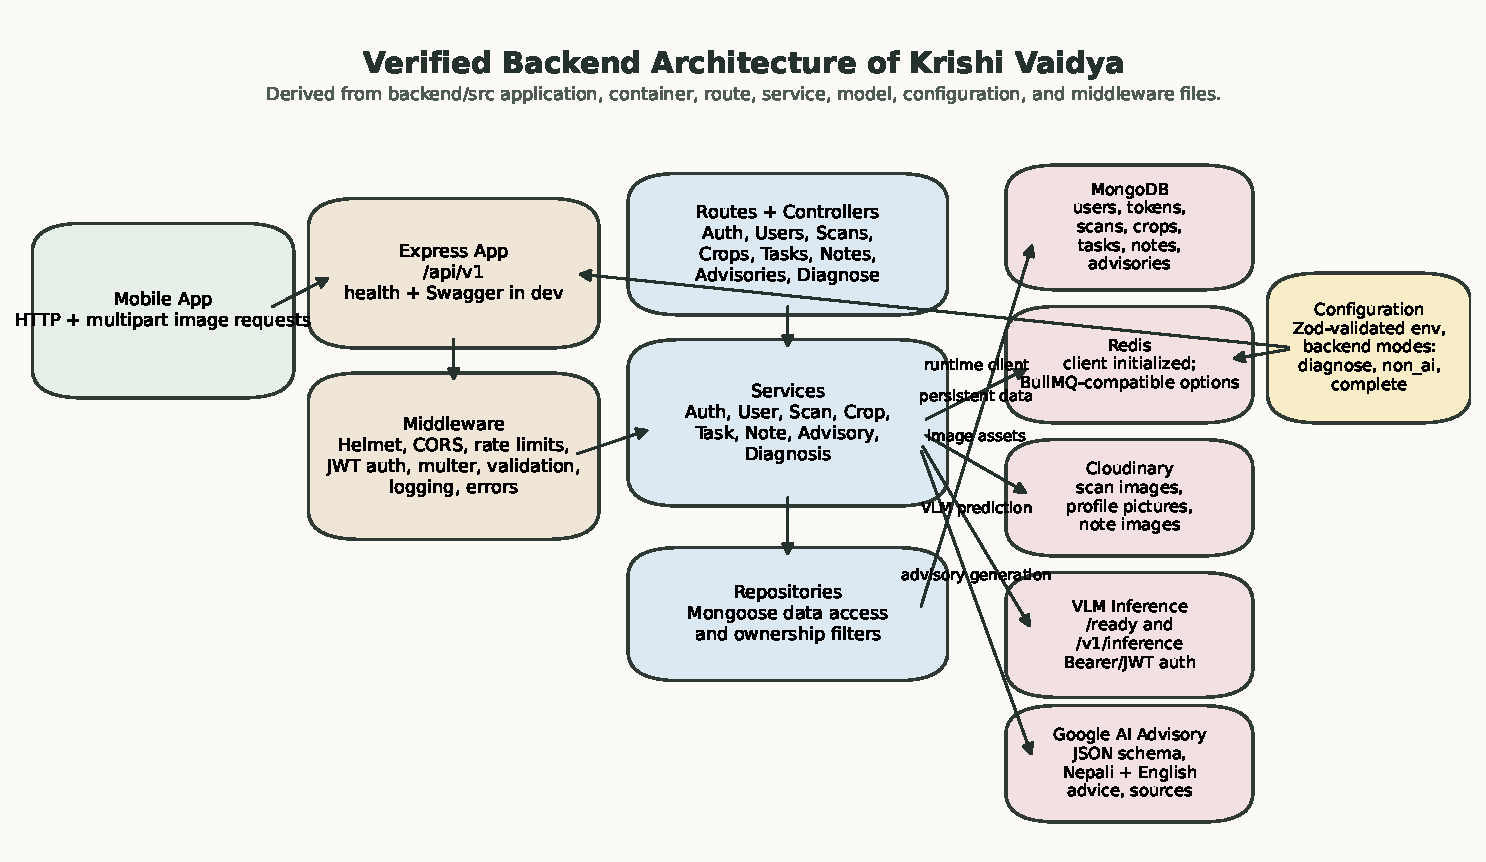
\includegraphics[width=\textwidth]{data/krishi_vaidya_backend_data/outputs/figures/backend_architecture.pdf}
\caption{Verified backend architecture of Krishi Vaidya}
\label{fig:backend-architecture}
\end{figure}

\ChapterSubsection{Runtime Modes and Application Initialization}

The Express application is created in \texttt{src/app.ts}. During initialization, the server sets
trust-proxy support, applies security middleware, applies CORS, applies the general rate limiter,
enables JSON and URL-encoded parsing with a 10 MB limit, and registers HTTP request logging. A
health endpoint is exposed at \texttt{/api/v1/health}; this endpoint reports server state such as
timestamp, uptime, environment, backend mode, server exposure mode, and the public base URL.

The backend supports three runtime modes through the validated \texttt{BACKEND\_MODE} environment
variable. In \texttt{diagnose} mode, only the diagnosis route is enabled. In \texttt{non\_ai} mode,
only database-backed routes are enabled. In \texttt{complete} mode, both the diagnosis route and
database-backed routes are enabled. This design is useful for development and deployment because
the AI diagnosis stack can be run separately from the full user-management and farm-management
stack when required.

\begin{table}[H]
\centering
\caption{Backend runtime modes and route availability}
\label{tab:backend-runtime-modes}
\begin{tabular}{@{}lll@{}}
\toprule
\textbf{Mode} & \textbf{Diagnosis route} & \textbf{Database-backed routes} \\
\midrule
\texttt{diagnose} & Enabled & Disabled \\
\texttt{non\_ai} & Disabled & Enabled \\
\texttt{complete} & Enabled & Enabled \\
\bottomrule
\end{tabular}
\end{table}

Configuration is validated with Zod before the server starts. The environment schema defines
server, MongoDB, Redis, JWT, Cloudinary, SMTP email, weather, ML-service, Google AI, and ngrok
settings. Required configuration depends on runtime mode: database-backed routes require JWT,
Cloudinary, and SMTP credentials, while the diagnosis stack requires the ML service URL and either
a bearer token or JWT private-key configuration when ML inference is enabled. This validation
prevents the server from silently starting in an incomplete state.

\ChapterSubsection{Dependency Container}

The backend constructs its dependencies in \texttt{src/container.ts}. Repositories are created
first, followed by services, controllers, and route modules. The container wires the authentication
service to the user, OTP, refresh-token, email, and user services; the scan service to scan,
scan-resolution, and file-upload dependencies; and the diagnosis service to validation, VLM
inference, and Google AI advisory clients. This explicit construction makes the dependency graph
visible and avoids scattering object creation across route files.

\ChapterSection{Backend API Design}

\ChapterSubsection{Route Groups}

The backend exposes versioned API routes under \texttt{/api/v1}. The implemented route groups are
authentication, users, scans, crops, tasks, notes, advisories, and diagnosis. The development
environment also serves OpenAPI documentation through Swagger UI at \texttt{/api/docs} and the
generated specification at \texttt{/api/docs.json}. Swagger comments in the route files document
request bodies, security requirements, path parameters, query parameters, and expected response
purposes.

\begin{table}[H]
\centering
\caption{Implemented backend route groups}
\label{tab:backend-route-groups}
\small
\resizebox{\textwidth}{!}{%
\begin{tabular}{@{}lll@{}}
\toprule
\textbf{Route group} & \textbf{Base path} & \textbf{Implemented responsibility} \\
\midrule
Health & \texttt{/api/v1/health} & Server status, runtime mode, uptime, and exposure information \\
Diagnosis & \texttt{/api/v1/diagnose} & Image validation, VLM inference request, advisory generation, diagnosis response \\
Authentication & \texttt{/api/v1/auth} & Registration, login, token refresh, logout, OTP, password reset \\
Users & \texttt{/api/v1/users} & Profile retrieval, profile update, profile image, password change, push tokens \\
Scans & \texttt{/api/v1/scans} & Scan upload, scan history, statistics, grouping, status, resolution, follow-up linkage \\
Crops & \texttt{/api/v1/crops} & Crop-plot creation, filtering, archive state, growth stage, health status \\
Tasks & \texttt{/api/v1/tasks} & Crop-task creation, batch creation, pending/overdue/upcoming views, completion state \\
Notes & \texttt{/api/v1/notes} & Crop notes, linked scan notes, note images, note-type counts \\
Advisories & \texttt{/api/v1/advisories} & Advisory creation, filtering, active advisories, dismiss/undismiss actions \\
\bottomrule
\end{tabular}%
}
\end{table}

\ChapterSubsection{Controller and Validation Pattern}

Controllers receive typed service dependencies and expose Express request handlers. Validation is
implemented with \texttt{express-validator} in the route/controller layer. Common validation
examples include MongoDB identifier checks for resource identifiers, bounded pagination values,
enumerated values for task categories, advisory severities, scan statuses, and crop stages, and
length limits for user text fields. The controllers format successful responses through a common
response formatter and pass operational failures to a global error middleware.

Most database-backed route groups require authentication. The authentication middleware checks a
Bearer access token, verifies the JWT with the configured secret, rejects expired or malformed
tokens, rejects pending-verification and blocked users, and attaches the decoded user context to
the Express request. This means service-layer methods can consistently receive the authenticated
user identifier and enforce ownership through repository queries.

\ChapterSection{Backend Data Model}

\ChapterSubsection{MongoDB Collections and Domain Entities}

The backend uses Mongoose models for persistent state. The implemented domain entities include
users, OTP records, refresh tokens, scans, scan resolutions, crop plots, crop tasks, crop notes,
and advisories. The models include indexes for common access paths such as user ownership,
status-based filtering, soft-delete filtering, date ordering, crop type, health status, task due
date, advisory severity, and TTL cleanup for expiring documents.

\begin{table}[H]
\centering
\caption{Implemented backend data models}
\label{tab:backend-data-models}
\small
\resizebox{\textwidth}{!}{%
\begin{tabular}{@{}lll@{}}
\toprule
\textbf{Model} & \textbf{Primary purpose} & \textbf{Important implementation details} \\
\midrule
\texttt{User} & User account and preferences & Email, password hash, name, language, region, accessibility, location, status, push tokens \\
\texttt{Otp} & OTP verification state & Purpose-specific OTP hash, attempt count, expiry, unique email-purpose index, TTL expiry \\
\texttt{RefreshToken} & Session refresh state & Token hash, lookup ID, device context, revocation state, expiry, TTL cleanup \\
\texttt{Scan} & Disease scan history & Image URI, crop metadata, status, result object, client timestamp, offline flag, soft delete \\
\texttt{ScanResolution} & Outcome tracking for scans & Resolution type, treatment used, notes, follow-up scan references \\
\texttt{CropPlot} & Farmer crop plot record & Crop type, variety, region, district, area, planting date, stage, health status, archive state \\
\texttt{CropTask} & Farm task and reminder record & Plot link, category, due date, priority, completion state, auto-generated flag \\
\texttt{CropNote} & Crop observation and treatment note & Plot link, optional scan link, note type, title/body, image attachments, soft delete \\
\texttt{Advisory} & Crop advisory notification & Plot link, advisory type, severity, Nepali/English fields, dismiss state, expiry TTL \\
\bottomrule
\end{tabular}%
}
\end{table}

\ChapterSubsection{Repository Layer}

The repository layer encapsulates database access. This is most visible in user-owned resources
such as scans, crop plots, tasks, notes, and advisories. Repository methods accept user identifiers
or plot identifiers and apply filters before returning results. This pattern reduces the risk of
accidentally exposing one user's records to another user because ownership filtering is part of
the data-access layer rather than being repeated manually in every controller.

\ChapterSection{Backend Diagnosis and Advisory Pipeline}

\ChapterSubsection{Image Validation}

The diagnosis route accepts a single image through the multipart field \texttt{image}. The
diagnosis validation service checks that the image exists, is non-empty, does not exceed the
configured maximum upload size, and is a valid JPEG, PNG, or WEBP file. The validation does not
trust the MIME type alone; it reads image headers and dimensions from the uploaded buffer. Images
smaller than \(64 \times 64\) pixels or larger than \(4096 \times 4096\) pixels are rejected.
The optional crop-name hint is also validated and limited to 80 characters.

\ChapterSubsection{VLM Inference Bridge}

After validation, the diagnosis service generates a request identifier and calls the VLM inference
client. Before inference, the client checks the VLM service readiness endpoint. The inference
request is sent to \texttt{/v1/inference} with base64 image data, media type, a deterministic
classification prompt, maximum token count of 320, temperature 0, and sampling disabled. The VLM
client supports static bearer-token authentication and RS256 JWT-based bearer-token generation
from configured private-key content or private-key path.

The VLM output is parsed as JSON when possible. If a JSON object is returned, the backend extracts
fields such as crop, disease, scientific name, canonical label, confidence, confidence label,
out-of-distribution flag, symptom descriptions, and alternatives. If the VLM output cannot be
parsed into JSON, the raw text is still preserved and passed forward as part of the advisory
generation context.

\ChapterSubsection{Google AI Advisory Bridge}

The backend then calls the Google AI advisory client. This client sends the uploaded image and the
parsed VLM prediction to Google AI Studio and requires the response to match a strict JSON schema.
The schema includes disease name, Nepali disease name, scientific name, crop, confidence,
confidence tier, out-of-distribution flag, symptom descriptions, treatment steps, prevention tips,
safety warnings, organic alternatives, source URLs, and optional alternative diagnoses. The system
prompt explicitly instructs the model to behave as an agricultural disease advisory expert for
farmers in Nepal, to use Nepali and English fields, to avoid unsafe pesticide advice, and to avoid
fabricated citations.

The advisory client can request Google Search grounding when enabled. If the selected model rejects
the search tool, the client retries without grounding using the configured fallback behavior. The
client validates the returned JSON using Zod before the diagnosis service returns the final API
response. The final response includes a request identifier, timestamp, disease fields, confidence
tier, out-of-distribution flag, symptom descriptions, advisory object, processing time, and a
model-version string composed from the VLM model and configured Google AI model.

\ChapterSection{Backend Security, Uploads, and Reliability Controls}

\ChapterSubsection{Authentication and Session Handling}

Authentication uses access tokens and refresh tokens. Registration creates a user account and the
login flow returns an access token while storing the refresh token in an HTTP-only cookie. Refresh
tokens are represented in the database as hashed token records with lookup identifiers, expiry, and
revocation state. The backend also supports logout from the current session and logout from all
devices.

OTP support is implemented for email verification, password reset, and phone verification
purposes. OTP records store hashes rather than plain OTP values and include expiry and attempt
tracking. The OTP collection has a unique email-purpose index and an expiry index, so each active
OTP purpose for an email has a controlled lifecycle.

\ChapterSubsection{Upload Handling and Cloudinary Storage}

The backend uses Multer memory storage for uploaded files. File filtering checks both MIME type and
extension against JPEG, PNG, and WEBP image formats. Scan images, profile pictures, and note images
are uploaded to Cloudinary through the file-upload service. The Cloudinary configuration applies
secure URLs and automatic quality/format transformations. The backend also supports deleting
Cloudinary assets when profile pictures or note images are replaced or removed.

\ChapterSubsection{Request Safety and Error Handling}

Request safety is handled through Helmet, CORS, rate limiting, validation, structured logging, and
a global error handler. The general rate limiter allows 100 requests per 15 minutes, authentication
routes allow 10 requests per 15 minutes, and OTP requests allow 5 requests per hour. The global
error handler converts known application errors, Multer upload errors, Mongoose validation errors,
duplicate-key errors, and JWT errors into consistent JSON error responses. In production, unknown
errors are hidden behind a generic internal-server-error message, while development mode exposes
more diagnostic detail.

\ChapterSection{Mobile Application Architecture}

\ChapterSubsection{Purpose and Implementation Scope}

The mobile application is the farmer-facing interface of Krishi Vaidya. It is implemented as an
Expo React Native application under \texttt{mobile\_app/app}. Its role is broader than image
capture alone: it provides onboarding, crop-plot management, scan capture, image review, diagnosis
submission, result presentation, local scan history, reminders, notifications, settings, data
export, and offline-aware operation. The application therefore acts as the field interface that
connects the trained model work and the backend API to a practical user workflow.
React Native and Expo support this cross-platform mobile implementation model
\parencite{reactNativeDocs,expoDocs}.

The implemented mobile project uses Expo Router as its routing layer, React Native as the runtime,
TanStack Query for server-state mutation handling, SQLite for local persistence, Zustand-style
stores for UI-facing state, i18next for bilingual text, VisionCamera for native capture, and
TFLite support for on-device inference assets. The application configuration declares Android
package \texttt{com.krishivaidya.app}, application scheme \texttt{krishivaidya}, portrait
orientation, camera and image-library permissions, typed routes, React Compiler support, and
environment-driven configuration for API base URL, API key, Sentry DSN, weather API key, and
feature flags.

Figure~\ref{fig:mobile-app-architecture} shows the implemented architecture. The diagram was
generated from the actual application structure rather than from an assumed design.

\begin{figure}[H]
\centering
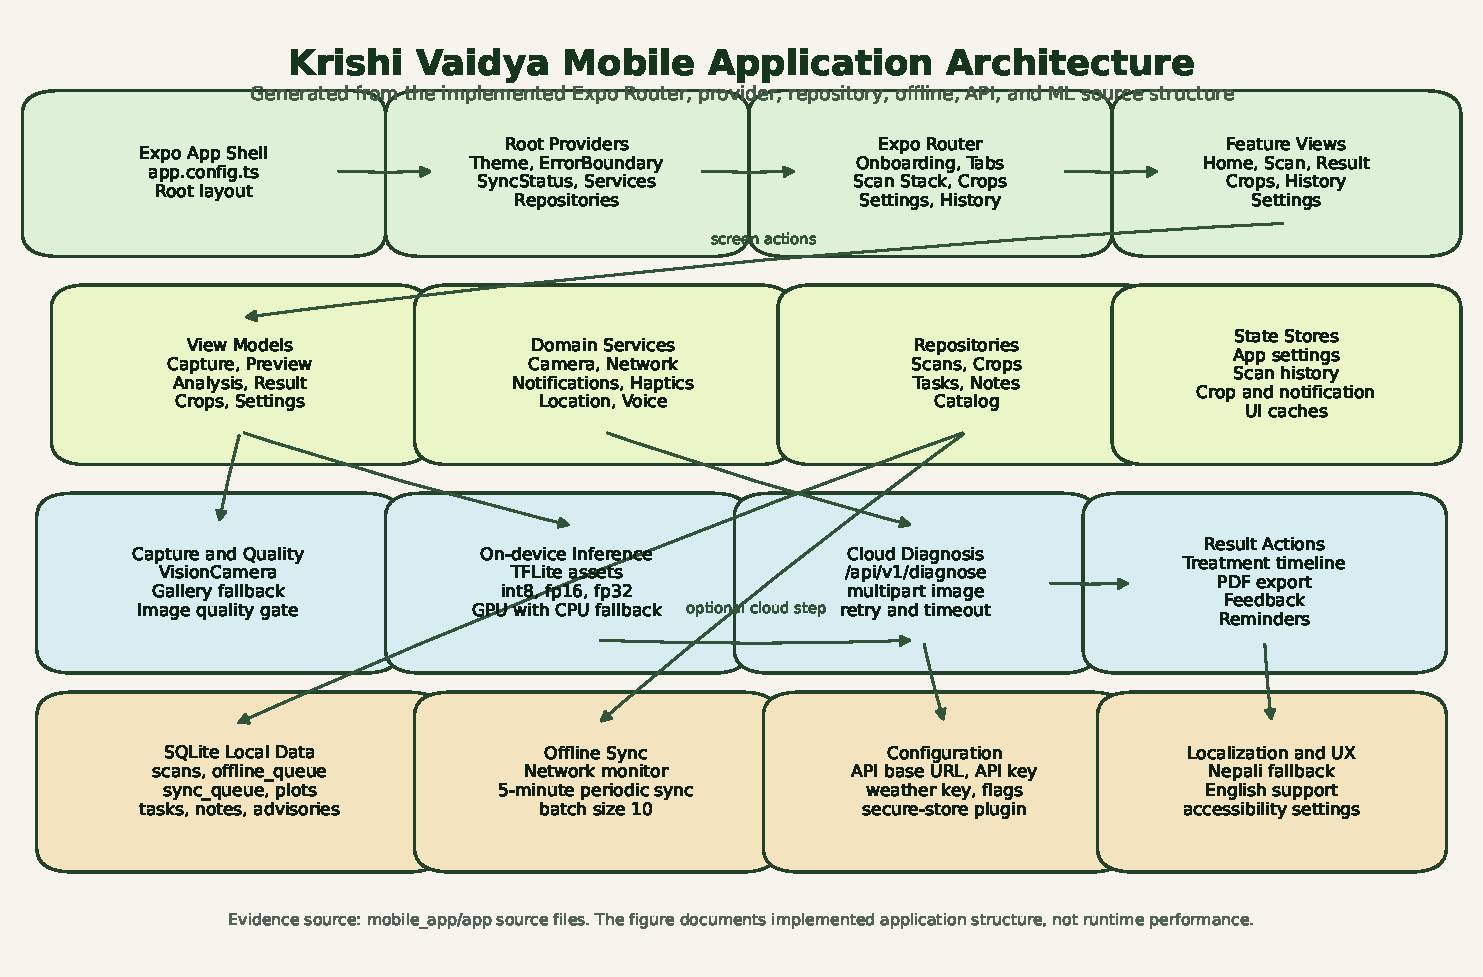
\includegraphics[width=\textwidth]{data/krishi_vaidya_mobile_app_data/outputs/figures/mobile_app_architecture.pdf}
\caption{Mobile application architecture generated from the implemented Expo, provider, repository, offline, API, and ML source structure.}
\label{fig:mobile-app-architecture}
\end{figure}

\ChapterSubsection{Application Shell and Navigation Structure}

The root application layout initializes the global runtime before the user reaches feature
screens. It loads fonts, controls the splash screen, creates a QueryClient with offline-tolerant
defaults, initializes i18n, wraps the application in theme, error-boundary, sync-status, service,
and repository providers, and bootstraps local repositories before rendering the route tree. It
also refreshes local crop, app-setting, and notification stores from SQLite and preloads the
TFLite service in the background. Route protection redirects users according to onboarding state,
so first-time users enter the onboarding flow before the main tab interface.

The implemented route hierarchy separates the application into onboarding routes, bottom-tab
routes, scan routes, crop-management routes, and settings routes. The bottom-tab navigator exposes
Home, Crops, Scan, History, and Settings as the primary farmer workflows. The scan stack contains
capture, preview, image-editor, analysis, and final-analysis screens. Crop-management routes
include crop creation, crop detail, editing, task creation, note creation, notes, tasks, and
weather. This structure keeps the scan workflow independent from longer-term farm-record
management while still allowing results and reminders to connect back to crop records.

\begin{table}[H]
\centering
\caption{Implemented mobile route and workflow groups}
\label{tab:mobile-route-groups}
\small
\resizebox{\textwidth}{!}{%
\begin{tabular}{@{}lll@{}}
\toprule
\textbf{Route group} & \textbf{Implemented screens} & \textbf{Primary purpose} \\
\midrule
Onboarding & Welcome, language, permission, crop, demo & First-run setup, language selection, permission preparation, crop context \\
Main tabs & Home, Crops, Scan, History, Settings & Primary application navigation for daily use \\
Scan stack & Capture, preview, image editor, analysis, final analysis & Image acquisition, review, detection, cloud diagnosis, report viewing \\
Crop routes & Add/edit crop, crop detail, crop weather, tasks, notes & Farm plot management and agronomic record keeping \\
Settings routes & Profile, option select, notifications, accessibility, export, model precision & Preference management, data export, accessibility, model deployment controls \\
Achievements & Achievements view and toast components & Lightweight engagement tracking based on completed app actions \\
\bottomrule
\end{tabular}%
}
\end{table}

\ChapterSubsection{Provider, Repository, and Dependency Structure}

The mobile app avoids constructing all dependencies directly inside screens. The
\texttt{ServicesProvider} exposes service abstractions such as camera, network, notification,
haptics, voice, and location services. The \texttt{RepositoryProvider} exposes repositories for
scans, crops, tasks, notes, and the data catalog. The repository bootstrap file is the central
construction point for local data sources and repositories. It initializes SQLite, runs the V3 to
V4 migration path, performs a one-time MMKV-to-SQLite migration, constructs local data sources,
creates repository instances, and initializes the offline sync manager.

This structure is important because it separates interface code from persistence and integration
details. Feature screens can call view models, view models can use repositories and services, and
repositories can use SQLite or fixture-backed catalog data without forcing the screens to know how
those dependencies are built. The project also keeps read-only agricultural catalog data separate
from mutable user records. Varieties, growth stages, fertilizer recommendations, disease catalog
entries, and seasonal tips are stored as fixtures, while user-created scans, plots, tasks, notes,
settings, achievements, and notifications are stored in SQLite.

\ChapterSubsection{Local Persistence and Offline-Aware Design}

The mobile data layer is built around a SQLite schema in which user-facing records are retained
locally. The implemented schema contains tables for scans, offline scan queue entries, reminders,
sync queue entries, crop plots, crop tasks, crop notes, crop advisories, custom task categories,
user settings, user achievements, achievement statistics, and notifications. Most mutable tables
include sync-related fields such as \texttt{sync\_status}, \texttt{updated\_at}, and
\texttt{deleted\_at}. This design supports local-first behavior because user actions can be stored
immediately on the device even when backend synchronization is delayed.

\begin{table}[H]
\centering
\caption{Implemented mobile local persistence groups}
\label{tab:mobile-local-persistence}
\small
\resizebox{\textwidth}{!}{%
\begin{tabular}{@{}lll@{}}
\toprule
\textbf{Persistence group} & \textbf{Tables or stores} & \textbf{Supported manuscript interpretation} \\
\midrule
Scan records & \texttt{scans}, \texttt{offline\_queue} & Local scan history, queued uploads, offline diagnosis fallback \\
Synchronization & \texttt{sync\_queue}, sync columns on mutable tables & Retryable operation queue and change tracking mechanism \\
Crop management & \texttt{crop\_plots}, \texttt{crop\_tasks}, \texttt{crop\_notes}, \texttt{crop\_advisories} & Farmer plot, task, note, and advisory records \\
Personalization & \texttt{user\_settings} & Language, theme, accessibility, onboarding, model precision, selected crops \\
Engagement and alerts & \texttt{user\_achievements}, \texttt{user\_achievement\_stats}, \texttt{notifications}, \texttt{reminders} & App engagement state, reminder scheduling, notification history \\
Catalog data & JSON fixture files through catalog repository & Read-only crop, growth-stage, fertilizer, disease, and seasonal reference data \\
\bottomrule
\end{tabular}%
}
\end{table}

The offline sync manager registers operation handlers, monitors connectivity, resets previously
interrupted processing items, listens for app-state changes, and starts a periodic sync timer with
a five-minute interval. Sync queue processing uses batches of ten items and stops when
connectivity is lost. The implementation already provides the synchronization mechanism, but the
source code also makes clear that some generic table-push behavior is currently represented by
marking local rows as synced until all matching backend endpoints are ready. Therefore, the mobile
manuscript should describe the offline sync system as implemented infrastructure with partial
backend push integration, not as fully proven two-way production synchronization.

\ChapterSubsection{Scan Workflow and Diagnosis Flow}

The scan workflow is implemented as a deliberate multi-stage process rather than as a single
button action. The native capture screen uses VisionCamera and supports model overlay state,
selected crop context, flash or torch control, focus and exposure behavior, zoom, camera switching,
photo capture, and gallery selection. A web-compatible capture view exists as a fallback path. The
preview stage reads image metadata and uses image-quality analysis to identify quality issues
before the user proceeds. The image-editor stage allows the captured image to be refined before
analysis.

The analysis view model implements an explicit state machine with phases \texttt{ready},
\texttt{scanning}, \texttt{reviewed}, \texttt{sending}, \texttt{success}, \texttt{failed}, and
\texttt{queued}. The scanning phase uses a pre-detection passed from capture when available, a
development mock only on web when enabled, or the inference service for image detection. The
disease-diagnosis phase calls the network-aware diagnosis hook. When online, the hook attempts
cloud diagnosis through the backend \texttt{/api/v1/diagnose} endpoint. When the connection is
slow, it races the cloud request against a five-second timeout and falls back if necessary. When
offline, it queues the scan and attempts to return cached advisory content if available.

The API client posts the selected image as multipart form data to \texttt{/api/v1/diagnose} with
an optional crop-name field. The client reads the base URL and optional API key from Expo
configuration, applies a bearer authorization header when configured, uses a 60-second diagnosis
timeout, logs requests and responses during development, and retries transient failures such as
timeouts, rate-limit responses, and server errors up to three times with exponential backoff.

\ChapterSubsection{On-Device Model Asset Support}

The mobile application includes native TFLite model support through a singleton TFLite service.
The implemented model asset map includes three precision variants:
\texttt{krishi\_bouncer\_int8.tflite}, \texttt{krishi\_bouncer\_fp16.tflite}, and
\texttt{krishi\_bouncer\_fp32.tflite}. The default input configuration is \(640 \times 640\), with
confidence threshold 0.35 and IoU threshold 0.45. The service reads the selected model precision
from app settings, attempts to load the model with an Android GPU delegate, and falls back to CPU
loading if the GPU delegate fails. It also exposes runtime precision switching and a benchmark
method that can load a chosen precision, run inference, and return load time and inference time.

One integration detail must be documented carefully. The YOLO manuscript section describes the
trained object detector and its class taxonomy from the YOLO training assets, while the mobile
TFLite service currently defines a disease-label list in source code. The manuscript should not
claim that this mobile TFLite asset has already been fully reconciled with the YOLO detector
taxonomy unless that alignment is separately verified. For this reason, the mobile section treats
TFLite support as implemented mobile inference infrastructure and identifies model-taxonomy
alignment as an integration verification item.

\ChapterSubsection{Localization, Accessibility, and Farmer-Facing Output}

The mobile application is designed as a Nepali-first interface with English support. The i18n
configuration first attempts to use the persisted SQLite language preference, then device locale,
and finally falls back to Nepali. The settings system includes language, region, theme, Wi-Fi-only
upload preference, haptics, reduced motion, voice output, high-contrast mode, large-text mode,
color-blind mode, user profile fields, selected crops, and model precision. Result presentation
includes treatment timeline support, organic alternative toggling, reminder creation, share-card
generation, PDF export, voice output, feedback submission, and navigation back to report history.

This design is significant for the final-year project because it positions Krishi Vaidya as an
applied agricultural decision-support system rather than only a model demonstration. The mobile app
contains the workflow required to move from image capture to diagnosis, advisory presentation,
follow-up actions, and longer-term crop records.

\ChapterSection{Integrated Diagnosis Workflow}

\ChapterSubsection{Integration Objective}

The integration layer connects the four implemented subsystems into one usable Krishi Vaidya
workflow. The YOLO and mobile inference assets support image-focused pre-analysis and mobile
deployment work. The VLM service provides crop-disease prediction from an image. The backend API
acts as the controlled orchestration layer between the mobile client, VLM inference gateway, and
advisory generator. The mobile app presents the result to the farmer and stores relevant local
state. The integration method therefore focuses on how an image moves through the system, how each
boundary validates or transforms the data, and how the final result becomes a farmer-facing
diagnosis and advisory report.

This section is deliberately separated from the individual component sections. The component
sections explain how each subsystem is built. The integration section explains how the subsystems
cooperate. Figure~\ref{fig:integration-workflow} summarizes the verified end-to-end diagnosis
flow from the implemented source files.

\begin{figure}[H]
\centering
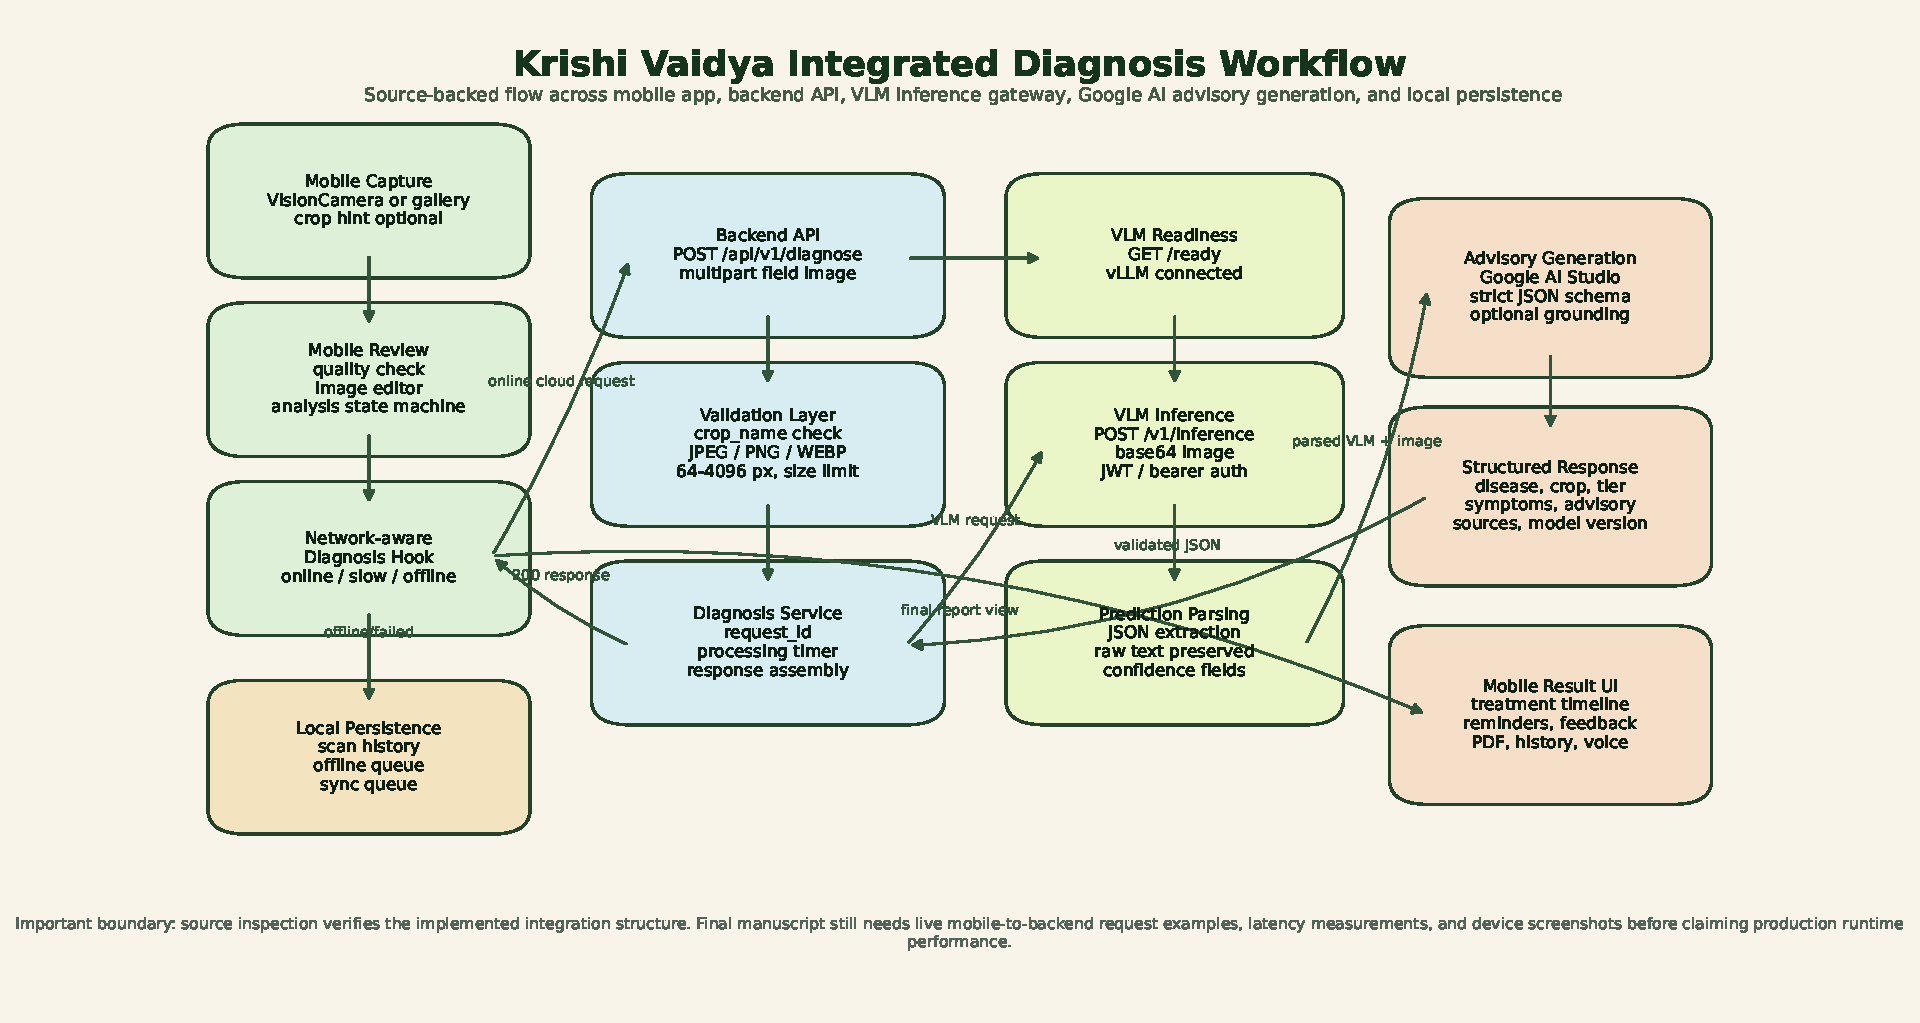
\includegraphics[width=\textwidth]{data/krishi_vaidya_integration_data/outputs/figures/integration_workflow.pdf}
\caption{Integrated Krishi Vaidya diagnosis workflow across mobile app, backend API, VLM inference gateway, advisory generation, and local persistence.}
\label{fig:integration-workflow}
\end{figure}

\ChapterSubsection{End-to-End Control Flow}

The implemented online diagnosis path starts in the mobile scan workflow. A user captures an image
with the native camera or selects an existing image from the gallery. The image passes through the
preview and image-editor stages before the analysis view model enters its diagnosis phase. At this
point, the network-aware diagnosis hook decides whether the request should be sent to the backend,
served from cached advisory data, or queued for later synchronization.

When the device is online, the mobile API client sends a multipart request to
\texttt{/api/v1/diagnose}. The image is sent in the multipart field \texttt{image}, and the app can
include an optional \texttt{crop\_name} field. The API client reads the backend base URL and
optional API key from Expo configuration, attaches a bearer authorization header when configured,
uses a 60-second timeout for diagnosis requests, and retries transient failures with exponential
backoff for status codes such as 408, 429, 500, 502, 503, and 504.

The backend route receives this request through the diagnosis route group. The route is exposed as
\texttt{POST /api/v1/diagnose} after the application-level route prefix is applied. The route uses
single-image upload middleware and delegates request processing to the diagnosis controller. The
controller does not implement diagnosis logic itself; it passes the uploaded file and optional
crop-name field into the diagnosis service and returns the service response as JSON.

\begin{table}[H]
\centering
\caption{Integrated online diagnosis control flow}
\label{tab:integration-control-flow}
\small
\resizebox{\textwidth}{!}{%
\begin{tabular}{@{}llll@{}}
\toprule
\textbf{Step} & \textbf{Source component} & \textbf{Implementation evidence} & \textbf{Output} \\
\midrule
1 & Mobile scan workflow & Capture, preview, editor, analysis view models & Image URI and optional crop context \\
2 & Mobile diagnosis hook & Network-aware mutation with online, slow, offline branches & Cloud request, cached result, or queued scan \\
3 & Mobile API client & Multipart \texttt{/api/v1/diagnose} request with retry and timeout & Backend diagnosis request \\
4 & Backend diagnosis route & Single-image upload middleware and diagnosis controller & Validated service input \\
5 & Backend validation & MIME, header, size, dimension, and crop-name checks & Validated image object \\
6 & VLM client & \texttt{/ready} then \texttt{/v1/inference} with prompt and bearer/JWT auth & Raw VLM prediction text and metadata \\
7 & Backend parser & JSON extraction with raw text preservation & Parsed VLM prediction context \\
8 & Advisory client & Google AI request with strict schema validation & Structured diagnosis and advisory payload \\
9 & Backend response assembly & Request ID, timing, confidence tier, model version & Application-facing JSON response \\
10 & Mobile result workflow & Result view model, history, reminders, feedback, PDF export & Farmer-facing report and local record \\
\bottomrule
\end{tabular}%
}
\end{table}

\ChapterSubsection{Backend Orchestration Boundary}

The backend is the central integration boundary because it protects the model and advisory
services from direct mobile exposure. The diagnosis service creates a request identifier, records
the processing start time, validates the optional crop name, and validates the uploaded image. The
image validator rejects missing images, empty images, files larger than the configured upload
limit, corrupt files, unsupported formats, MIME mismatches, images smaller than \(64 \times 64\)
pixels, and images larger than \(4096 \times 4096\) pixels. It supports JPEG, PNG, and WEBP image
formats.

After validation, the backend calls the VLM inference client. The client first checks the VLM
gateway readiness endpoint \texttt{/ready}. If the VLM service is not configured, not ready, times
out, or is unreachable, the backend raises a service-unavailable error rather than sending an
uncontrolled partial result to the mobile app. If the VLM service is ready, the backend posts to
\texttt{/v1/inference} with base64 image data, media type, deterministic generation settings,
maximum token count of 320, request ID, and a compact crop-disease JSON prompt. The prompt treats
the mobile crop name as a hint, not as a fact, and asks for fields such as crop, disease,
Nepali disease name, scientific name, confidence, confidence label, out-of-distribution state,
symptom descriptions, and alternatives.

Authentication between the backend and VLM service supports two modes. If a static bearer token is
configured, the client sends that token. Otherwise, when private-key material is configured, the
client generates an RS256 JWT with issuer, audience, subject, scope, expiry, and token identifier.
The generated token is cached until near expiry. This matters for the integration design because
it avoids placing VLM service credentials in the mobile application and keeps inference access
behind the backend boundary.

\ChapterSubsection{VLM Inference Gateway Boundary}

The VLM inference gateway is implemented as a FastAPI service, using a Python API framework based
on standard type hints \parencite{fastapiDocs}. It exposes a liveness endpoint
\texttt{/health}, a readiness endpoint \texttt{/ready}, and the inference endpoint
\texttt{/v1/inference}. Readiness succeeds only when the gateway has a vLLM client and the vLLM
backend reports the expected model as reachable. Inference requests require JWT authentication and
the correct \texttt{inference} scope. The request schema requires an image source and supports
either base64 image data or a public image URL, but not both in the same request.

The gateway validates image data before forwarding it to vLLM. For the backend integration path,
the image arrives as base64. The VLM gateway validates the image according to configured size,
dimension, allowed-format, and visual-token limits. It then forwards validated image bytes and the
prompt to the vLLM client. The response returned to the backend contains the request identifier,
prediction text, latency in milliseconds, input-token count, output-token count, model identifier,
and timestamp. The prediction text is normally expected to be JSON, but the backend does not trust
that assumption blindly.

\ChapterSubsection{Prediction Parsing and Advisory Generation}

The backend parses the VLM prediction in a defensive way. It first tries to parse the complete
prediction as JSON. If that fails, it attempts to extract the first JSON object embedded inside the
text. If no valid JSON object can be extracted, the backend preserves the raw VLM text. When JSON
is available, the backend extracts fields such as crop, disease, disease Nepali name, scientific
name, canonical label, confidence, confidence label, out-of-distribution flag, symptom
descriptions, and alternatives. Numeric confidence values are clamped between 0 and 1, and
alternatives are limited to at most three items.

The parsed or raw VLM output is then passed to the Google AI advisory client along with the
validated image. The advisory client instructs the model to behave as an agricultural disease
advisory expert for farmers in Nepal, to use Nepali and English fields, to avoid fabricated
citations, and to avoid unsafe pesticide advice. The request can include Google Search grounding
when enabled. If the selected model rejects the grounding tool, the client retries without
grounding according to the configured fallback behavior. The response must match a Zod-validated
schema before it is accepted.

\begin{table}[H]
\centering
\caption{Integrated data contract across diagnosis boundaries}
\label{tab:integration-data-contract}
\small
\resizebox{\textwidth}{!}{%
\begin{tabular}{@{}llll@{}}
\toprule
\textbf{Boundary} & \textbf{Input} & \textbf{Validation or transformation} & \textbf{Output} \\
\midrule
Mobile to backend & Multipart image, optional crop name & URI check on client; file upload middleware on server & Express file and crop-name value \\
Backend validation & Uploaded image buffer & MIME/header/dimension/size checks; crop-name validation & Validated image and optional crop hint \\
Backend to VLM gateway & Base64 image, media type, prompt, request ID & Readiness check, timeout, bearer/JWT auth & VLM inference request \\
VLM gateway to vLLM & Validated image bytes and prompt & JWT scope, image validation, rate limit, vLLM health & Prediction text and inference metadata \\
Backend parser & VLM prediction text & JSON parse, embedded JSON extraction, raw-text fallback & Parsed VLM context \\
Backend to advisory model & Image and parsed VLM context & Strict system prompt, schema request, retry/fallback & Structured advisory payload \\
Backend to mobile & Diagnosis response JSON & Confidence-tier calculation, alternative filtering, model-version assembly & Farmer-facing diagnosis response \\
Mobile result view & Structured response JSON & Bilingual field selection, timeline mapping, local history save & Report, reminders, feedback, export paths \\
\bottomrule
\end{tabular}%
}
\end{table}

\ChapterSubsection{Mobile Offline and Slow-Network Integration}

The mobile app includes separate behavior for online, slow, and offline states. When network status
is online, it attempts the cloud diagnosis request. If that request fails, it falls back to the
offline queue path. When network status is slow, it races the cloud diagnosis request against a
five-second timeout and falls back if the request does not complete in time. When the device is
offline, it does not attempt the backend call and instead queues the scan directly.

Queued scans are written to the SQLite-backed offline queue and also inserted into the main scan
history as pending offline scans. The queue manager also enqueues a high-priority
\texttt{scan\_diagnosis} item in the unified sync queue. If a matching cached advisory is
available, the diagnosis hook can return cached advisory content immediately while still keeping
the scan queued for future cloud diagnosis. This behavior is important for field use because it
prevents the app from becoming useless when network connectivity is unavailable.

\ChapterSubsection{Structured Response and Farmer-Facing Output}

The backend returns a structured diagnosis response rather than exposing raw VLM text. The response
contains request ID, timestamp, disease, Nepali disease name, scientific name, crop, numeric
confidence, confidence tier, out-of-distribution flag, symptom descriptions, advisory details,
processing time, and model version. Alternatives are included only for medium- or low-confidence
responses. The confidence-tier calculation marks a response as out-of-distribution if the advisory
model marks it out of distribution or if confidence is below 0.30. Confidence values of at least
0.85 are high, values from 0.60 to below 0.85 are medium, and lower non-OOD values are low.

The mobile result view consumes this structured response. It selects Nepali or English disease
names according to current language, maps treatment steps into a timeline, supports organic
alternative toggling, allows feedback submission, opens reminder creation, supports share-card and
PDF export behavior, triggers voice output, and saves completed scans to local history. Therefore,
the integration output is not only a class label. It is a complete advisory object that can be
displayed, stored, revisited, exported, and used for follow-up actions.

\ChapterSubsection{Integration Verification Boundary}

The integration workflow is source-verified, but not yet fully runtime-verified in the manuscript.
Source inspection confirms the route contracts, validation checks, inference gateway contract,
advisory schema validation, mobile network branches, offline queueing, and result-display mapping.
The available VLM API tests also cover health readiness, authentication requirement, bad-scope
rejection, invalid-image rejection, successful inference response mapping, vLLM error mapping, and
rate-limit behavior. However, the final thesis should still add live mobile-to-backend request
examples, emulator or physical-device screenshots, measured latency, and an offline-to-online
sync demonstration before making production-readiness claims.

\ChapterSection{Testing and Validation}

\ChapterSubsection{Validation Strategy}

Testing and validation for Krishi Vaidya were organized around the actual structure of the system.
The project is not validated by one metric alone because it contains trained models, an inference
gateway, a backend API, a mobile application, and an integrated diagnosis workflow. Therefore, the
validation strategy separates five kinds of evidence: model-performance validation, dataset and
pipeline integrity checks, automated backend/API tests, mobile source and inference checks, and
integration-boundary verification.

This separation is important for accuracy. A high YOLO score does not prove that the backend is
correct. A passing backend scan test does not prove that the mobile app works on a physical
device. A valid VLM inference API test does not prove that the model predictions are accurate.
The manuscript therefore treats each validation result according to what it actually verifies.
Figure~\ref{fig:validation-coverage} summarizes the validation coverage and the remaining
evidence gaps.

\begin{figure}[H]
\centering
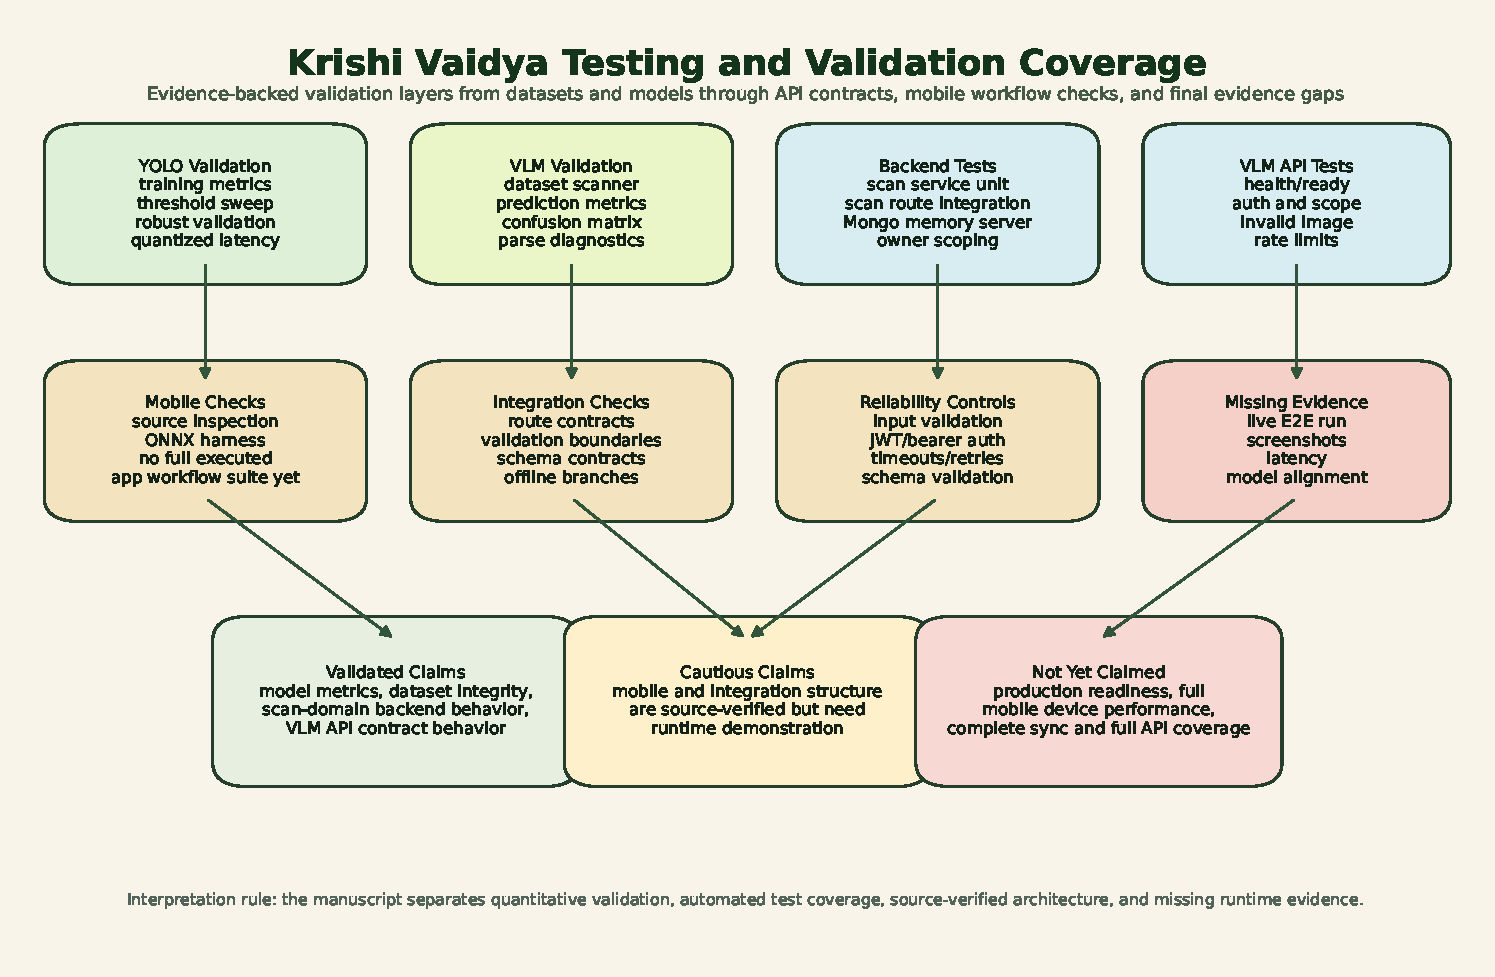
\includegraphics[width=\textwidth]{data/krishi_vaidya_validation_data/outputs/figures/validation_coverage.pdf}
\caption{Testing and validation coverage across model, backend, mobile, API, and integration layers.}
\label{fig:validation-coverage}
\end{figure}

\ChapterSubsection{YOLO Validation}

The YOLO subsystem has the strongest quantitative detection evidence in the project. Its
validation includes training dynamics, best-epoch metrics, robust validation on the validation
split, threshold analysis, quantized model comparison, per-class metrics, latency measurements,
confusion matrix outputs, and error-category analysis. The validation artifacts are stored under
the YOLO result directories and were converted into manuscript-ready figures and tables in the
YOLO manuscript data folder.

The YOLO training metrics show the training trajectory across 100 epochs. The best recorded
training summary used in the manuscript reports precision 0.71717, recall 0.74868, mAP50
0.76163, and mAP50-95 0.60191 at epoch 100. Robust validation provides an additional evaluation
view using the validation images and labels. In the baseline robust-validation summary, 3,527
images and 20,443 ground-truth objects were evaluated, producing 3,701 true positives, 171 false
positives, and 16,742 false negatives at confidence threshold 0.25 and IoU threshold 0.5. This
corresponds to precision 0.69286, recall 0.79522, F1 0.74016, and mean inference time
12.609 ms in that validation run.

The YOLO validation scripts also have automated tests for the validation pipeline itself. These
tests verify data-YAML loading, image collection, normalized-label conversion, IoU computation,
prediction-ground-truth matching, class-aware matching, argument/config resolution, validation
state-machine step selection, validation command execution wiring, dataset provisioning, training
manifest creation, quantization manifest behavior, model-validation manifest behavior, packaging
manifest behavior, launch smoke behavior, and resume behavior. These tests support the reliability
of the validation tooling, while the quantitative result files support the detector-performance
claims.

\ChapterSubsection{VLM Validation}

The VLM subsystem was validated at two levels: dataset/pipeline validation and prediction
validation. Dataset validation checked the prepared Qwen-format records and image references. The
recorded dataset-validation summary reports 13,294 images found, 6,647 Qwen records, zero decode
failures, zero missing Qwen images, and zero recorded issues. This supports the claim that the
exported VLM dataset was structurally usable for training and evaluation.

Prediction validation was more severe. The independent test split contained 798 examples across
13 classes. The recorded prediction metrics report accuracy 0.13033, macro precision 0.52317,
macro recall 0.18342, macro F1 0.24655, and 540 parse-error predictions. These values are already
discussed in the VLM results section, but they are repeated here as validation evidence because
they define the current reliability boundary of the VLM component. The validation does not support
a claim that the current fine-tuned VLM is already diagnostically strong. It supports a more
careful claim: the VLM training and evaluation pipeline exists, the dataset export is structurally
validated, and the current model behavior exposes a serious parseability and prediction-quality
limitation that the final system must acknowledge.

The VLM repository also contains automated tests for dataset normalization, deduplication, source
adapters, split creation, manifest behavior, training data loading, training runtime compatibility,
runtime accelerator configuration, inference runtime configuration, inference batching,
performance batch-size resolution, validation metric calculation, prediction parsing, and the
FastAPI inference gateway. Across the visible VLM test files, there are 46 Python test functions,
including 11 tests dedicated to the inference API route behavior.

\ChapterSubsection{VLM Inference API Validation}

The VLM inference gateway has a focused API test suite. These tests use a stubbed vLLM client and
FastAPI test client rather than loading the full model. This is appropriate for route-contract
validation because the purpose is to verify HTTP behavior, authentication handling, request
validation, and error mapping without requiring GPU inference in the test process.

The inference API tests cover liveness, readiness failure, readiness success, missing
authentication, insufficient JWT scope, invalid base64 image rejection, successful inference
response mapping, timeout/unreachable/backend-failure mapping, environment setting loading,
settings-cache overrides, and configured rate-limit behavior. This gives the manuscript concrete
evidence that the inference gateway is not only a conceptual endpoint. Its API contract and
failure behavior are represented in automated tests.

\ChapterSubsection{Backend Validation}

The backend validation evidence is strongest for the scan domain. The available unit tests focus
on the scan service, and the integration tests focus on scan routes. The test setup uses
MongoDB Memory Server, clears database collections between tests, and configures test environment
variables for JWT, Cloudinary, Redis, email, MongoDB, and server port. This allows scan behavior
to be tested without depending on a persistent external MongoDB instance.

The scan service unit tests cover scan creation, offline scan creation, owner-scoped retrieval,
non-existent scan handling, cross-user access protection, pagination, status filtering,
crop-type filtering, update behavior, soft deletion, statistics, resolution creation, duplicate
resolution rejection, resolution retrieval, follow-up linkage, related scans, and grouping. The
scan route integration tests cover authentication requirement, paginated retrieval, filtering,
pagination, statistics, grouping, invalid group-by validation, scan lookup, missing-scan behavior,
status retrieval, resolution creation, duplicate-resolution protection, follow-up linkage, and
related-scan lookup.

There are 21 visible scan-service unit test cases and 26 visible scan-route integration test cases.
This is meaningful evidence for the scan domain, but it is not complete backend coverage.
Equivalent test evidence is not yet visible for every authentication, crop, task, note, advisory,
diagnosis, VLM-client, Google-advisory-client, and upload-validation path. Therefore, the backend
should be described as partially automated-tested, with scan behavior well represented and broader
route-domain tests still required before claiming full backend verification.

\ChapterSubsection{Mobile Validation}

The mobile application currently has source-level and harness-level evidence, but it does not yet
have complete automated workflow evidence. Source inspection verifies the route hierarchy,
provider setup, repository bootstrap, SQLite schema, offline queue, sync manager, diagnosis hook,
API client, result view model, settings, localization, and model-asset loading paths. This is
enough to document the implemented architecture, but it does not prove physical-device behavior.

The visible mobile test evidence is an ONNX YOLO engine test harness. It provides utilities for
model loading, warmup, dummy-image inference, detection validation, inference-result validation,
and full test-suite execution. However, it is a harness rather than evidence of a complete
executed mobile app test suite. The mobile manuscript should therefore avoid claiming full
app-level validation until an emulator or physical-device run is recorded. The remaining evidence
should include screen screenshots, camera behavior, TFLite loading behavior, mobile-to-backend
request timing, result-screen rendering, offline queue behavior, and recovery after network
restoration.

\ChapterSubsection{Integration Validation}

Integration validation is currently source-verified and contract-described rather than fully
runtime-demonstrated. The source confirms the mobile-to-backend route contract, backend upload
validation, backend-to-VLM readiness and inference calls, VLM gateway authentication and image
validation, backend VLM prediction parsing, advisory schema validation, structured response
assembly, mobile result mapping, and offline queueing. The generated integration diagram and
integration tables document those boundaries.

The final missing step is live end-to-end validation. A complete final validation pass should run
the mobile app against a configured backend and VLM gateway, capture a real diagnosis request,
record the backend response JSON, collect backend and VLM logs, measure latency, verify the result
screen, and test offline-to-online recovery. Until that evidence is added, the manuscript should
state that the integration workflow is implemented and source-verified, not that it has been
fully production-validated.

\begin{table}[H]
\centering
\caption{Testing and validation evidence summary}
\label{tab:testing-validation-summary}
\small
\resizebox{\textwidth}{!}{%
\begin{tabular}{@{}llll@{}}
\toprule
\textbf{Area} & \textbf{Evidence available} & \textbf{What it supports} & \textbf{Remaining gap} \\
\midrule
YOLO & Training, robust validation, threshold, quantization, latency, error outputs; validation-tool tests & Detector-performance and deployment-tradeoff claims & Direct mobile-device detector profiling \\
VLM & Dataset validation, prediction metrics, confusion matrix, parse diagnostics; 46 visible Python tests & Dataset integrity and honest VLM limitation claims & Model improvement and stricter output-format reliability \\
VLM API & 11 visible inference API tests & Health/readiness/auth/validation/error/limit contract claims & Live GPU-backed endpoint logs and latency \\
Backend & Scan service and scan route tests with MongoDB memory server & Scan-domain service and route behavior claims & Auth/crop/task/note/advisory/diagnosis test expansion \\
Mobile app & Source verification and ONNX inference harness & Architecture and planned inference-check claims & Executed emulator/device workflow tests and screenshots \\
Integration & Source-verified route and schema contracts & Implemented workflow boundary claims & Live end-to-end request, response, latency, and offline recovery evidence \\
\bottomrule
\end{tabular}%
}
\end{table}
